\chapter{Introduction}
\label{chap1}
\vspace{-1.5\baselineskip}
\section{Problem statement}
The human brain is organized into distributed functional modules that work
independently for specific cognitive tasks, and also interact with each
other. It has been shown that the spontaneous fluctuation of the blood
oxygenation level dependent (BOLD) signal, as measured by functional magnetic
resonance imaging (fMRI), is a valuable data source for delineating the
functional network organization. More recently, the spontaneous activity of
human brain has gained more attention because of its potential in helping understand
the \emph{baseline} patterns of cognitive activity as well as the cause of some
cognitive diseases. Resting-state fMRI (rs-fMRI) is accordingly widely used for
exploring such activities.

The analysis of rs-fMRI data is a challenging task, due to the scanner noise,
physiological noise, head motion, and subject's random thoughts during data
acquisition. Single subject's data are typically unreliable and inconsistent for
the statistical inference of the whole population's intrinsic activity patterns.
On the other hand, combining data from multiple subjects and jointly estimating
the common functional networks is more robust. In group analysis of rs-fMRI
data, one typically assumes that all subjects in the group share common
functional connectivity patterns, These group networks can be estimated more
accurately because the noise introduced in each subject is canceled by
averaging. In practice, it is a major challenge to summarize the consistent
patterns across subjects, as each subject's network patterns appear similar but
have slight variation due to the anatomical and functional difference across
subjects.

Recent years have seen substantial interest in estimating functional networks of
individual subjects during group analysis. An accurate estimate of an
individual's network is an important step towards understanding of
brain-behavior relationships on a per-subject basis. The intersubject variation
must be accounted for in order to obtain a good estimation of the networks of
individual subjects as well as the group.  Current
methods~\cite{yeo2011organization,damoiseaux2006consistent} either do not
estimate individual functional network maps, or do not have an explicit statistical
model on the intersubject variations~\cite{calhoun2001method,
  calhoun2001spatial}.  Among the methods that do estimate subject functional
networks, some have one or more of the drawbacks.

First, some methods map a common group functional network by concatenating the
BOLD signal from all subjects. By doing this, one implicitly assumes that the
voxels across subjects map to the same anatomical structure after
coregistration, and share the same functional connectivity patterns. These
assumptions are often violated due to the anatomical inhomogeneity between
subjects, and also due to the imperfect alignment of the existing coregistration
routine. In addition, the simple concatenation does not take into account the
possible different variance across subjects. In particular, some participants
may experience spontaneous, but active cognition during the scan even in the
resting-state. These activities modulate each subject's functional network in a
different way and to a different extent, and hence tamper the estimation of the
group's functional networks. Such subject-specific confounding factors are less
likely to be negligible by simple averaging compared to other sources of noise
such as scanner noise, subject motion and coregistration.

Second, group analysis are often conducted in a \emph{one way} procedure. In
some scenarios~\cite{van2008normalized,craddock2012whole,greicius2004default,
  greicius2007resting,seeley2009neurodegenerative,mohammadi2009changes}, each
subject's functional network is estimated independently, and a group map is
simply summarized by averaging the subjects' connectivity maps. The estimates of
subject maps by these procedures do not use other subjects' information and are
robust to noise. The group summary map extracted from these subject maps is
hence suboptimal. In other scenarios~\cite{calhoun2001method}, a group map is
estimated first from the concatenated data, then is back-reconstructed to obtain
the subject network maps. More recently, the subject network maps are estimated
from the averaged group map using a dual regression
approach~\cite{filippini2009distinct,beckmann2009group}. Such methods treat
voxel intensity from all subjects the same way for group map estimation,
ignoring that they may have subject specific variances. Both classes of approach
do not iteratively refine the initial group or subject estimates, and the
estimation of one subject's connectivity does not benefit from the information
obtained from other subjects. Figure \ref{fig:bidirections} gives an
illustration of the various methods and their order of estimations.

Last, spatial smoothing is often used during preprocessing in order to address
the issue of imperfect intersubject alignment. Although spatially blurring the
time series increases the signal-to-noise ratio, the choice of the smoothing
kernel size has a big impact on the estimated functional maps. Over-smoothing
inevitably results in the loss of fine structures of the functional maps. In
practice, the random field theory of statistical parametric mapping (SPM)
\cite{friston2007statistical} requires a smoothing kernel even larger than the
anticipated region of interest. One needs a model that uses the spatial
dependency and the intersubject similarity of the rs-fMRI signals, without
losing the finer details of the functional patterns.

A data-driven, unified probabilistic framework will help in solving the above
issues. The model should integrate both group's and subjects' connectivity
variables into this model. One can make inference from the posterior
distribution of the variables in both subject and group levels given the
observed BOLD signal.

In this dissertation we present a series of statistical methods for identification of
the human brain's functional networks by using rs-fMRI data. All the methods
aim to model the spatial dependency within a single subject in a principal way
without the naive spatial smoothing, and model the intersubject similarity and
variations for a more accurate group and subject network estimation. The main
mathematical tools are Markov random fields (MRF) --- an undirected graphical
model, and Bayesian method.  We use various methods including Markov chain Monte
Carlo (MCMC) sampling and variational inference for solving the statistical
inference problem in high dimensional space.

% Goal of this thesis.
\section{Disserattion statement}
Here is the statement of this dissertation:
\begin{center}
\parbox{5in}{\emph{A multilevel Markov Random Field model improves the
    reliability of the functional network estimation in rs-fMRI group study by
    taking into account context information as a prior. The data-driven Bayesian
    model can jointly estimate both population and subjects' connectivity
    networks, as well as drawing inference on the uncertainty in the estimation,
    and on the variability across subjects. }}
\end{center}

\noindent The word \emph{Context} has two meanings: 1) The functional patterns
of the human brain are spatially coherent. Neighboring voxels have larger probability
of being in the same functional network. 2) The network that a voxel belongs to
in one subject is dependent on the networks of the same voxels in other
subjects. The patterns of functional networks from the rs-fMRI study are to some
extent shared by multiple subjects, while the variability across subjects must
be taken into account.

By \emph{reliability} we mean the decrease in the variance of the functional
networks that we estimate with different subsets of all subjects. The reliable
estimates will be closer to the true network in the simulation test, where we
know the true answer.

To test our statement, we propose the following contributions:
\begin{itemize}
  \item \textbf{Full airwise connectivity with spatial coherence.} We propose a
    method that estimates pairwise functional connectivity in the whole brain of
    a single subject, without \emph{a priori} knowledge of the seed region. The
    model needs to take into account the spatial context information, and learn
    the strength of the coherence from the data.

  \item \textbf{Identify consistent, spatially coherent multiple functional
    networks.} We propose a data-driven, generative model that can cluster the
    gray matter voxels of a single subject's brain into disjoint multiple
    functional networks, while respecting the spatial coherence of the voxels.

  \item \textbf{Hierarchical model for group study.} We propose a hierarchical
    model that can estimate functional networks from a group of subjects. The
    model will estimate an overall group's network map as well as individual
    subjects network maps at the same time. When clustering the voxels into
    different networks, spatial neighbors both within and across subjects will
    be used in a prior distribution of a Bayesian framework. The variability of
    each subject's connectivity due to noise and artifact will be reduced to the
    extent that is to be determined automatically from the data.

  \item \textbf{Variability of resting-state functional network. } Based on
    the hierarchical MRF model proposed above, we will draw inference on the
    variance and the confidence intervals of the functional network. we will
    test the variability of the network by using a subset of the data and
    perform bootstrap sampling. we also explore and visualize the modes of
    spatial variability of the functional network patterns.
\end{itemize}

\section{Outline and contributions}
The remainder of the dissertation is organized in the following chapters. 

In Chapter \ref{chap:bg}, we will give a survey of the existing methods of
modeling the brain's functional connectivities using rs-fMRI, as well as the
statistical inference methods. we will describe the similarities and differences
across these varied statistical approaches, evaluate their advantages and
disadvantages, and relate them with our model.

Chapter \ref{chap:math} gives a general introduction of the mathematical tools
that will be used in the following chapters. These tools include graph,
graphical models and MRF, and various statistical inference methods including
sampling, variational Bayesian, graph cuts and other approximation methods.

Chapter \ref{chap:method1} will discover the first method that estimates a single
subject's functional networks. This chapter is an application of the graphical
model and MRF that we introduce in Chapter \ref{chap:math}. In this particular
case, the MRF is in a high dimensional space to model the prior distribution of
the pairwise connectivity variables. Also, we use variational inference to solve
the problem. The inference is implemented on graphical processing unit (GPU) to
speed up such a problem with $N^2$ complexity.

In Chapter \ref{chap:method2}, we apply the graphical model in  different
settings. Here the model is defined on the voxels in an original image domain
instead of on the higher dimensional domain defined in previous chapter. Together with a
mixture model and Bayesian method, we estimate all functional networks of a
single subject dataset with spatial regularization.

Chapter \ref{chap:method3} extends the concept of the graph to multiple
subjects, and estimate the functional patterns with a group of rs-fMRI
data. Both group and subject functional networks are estimated with higher
accuracy, better consistency than standard methods. This chapter will also cover
the validation of the hierarchical model. Besides the estimation accuracy, we
focus on the consistency of the method across multiple sessions, and also under
data perturbation.

Chapter \ref{chap:alldiscussion} concludes the dissertation with a general
discussion, and some future work that is worthy to explore.

\begin{figure}[p]
  \centering
  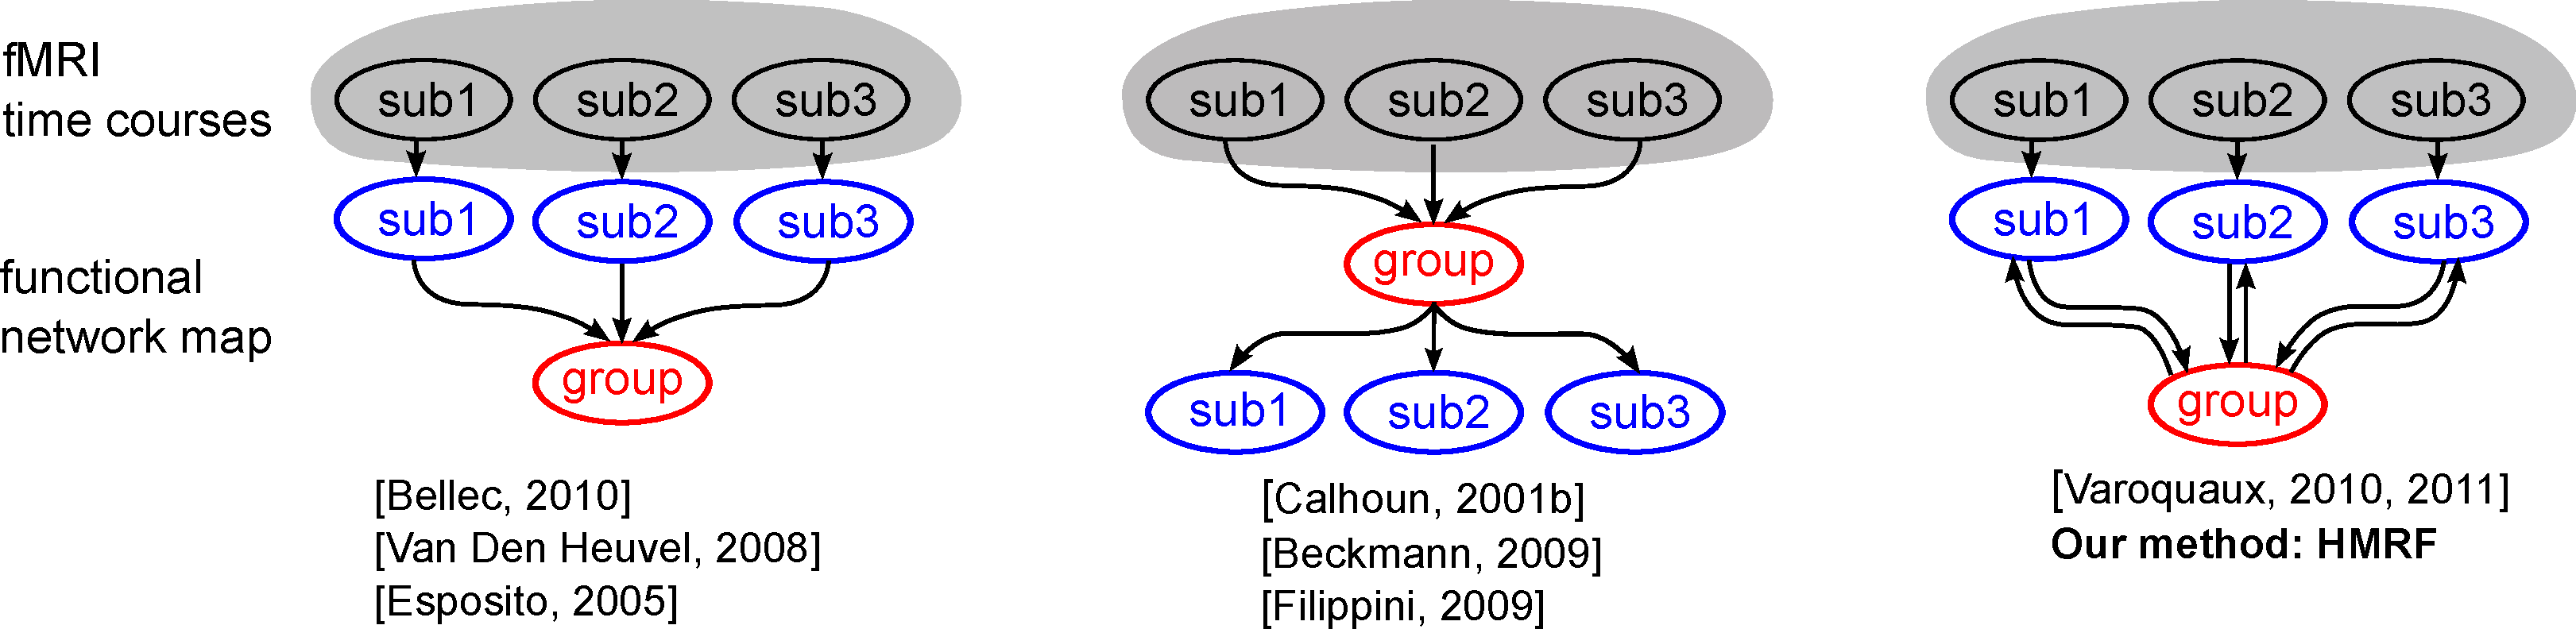
\includegraphics[width=0.9\textwidth]{figures/c1/bidirections}
  \caption{The order of estimation of various methods in group analysis.}
  \label{fig:bidirections}
\end{figure}

%%% Local Variables: 
%%% mode: latex
%%% TeX-master: "MyThesis"
%%% End:
